% ==============================================================================
% Chapter 5: Mathematical Models, Algorithms & Quantitative Simulations
% ==============================================================================
\chapter{מודלים מתמטיים, אלגוריתמיקה וסימולציות כמותיות ב-Python}
\label{ch:math}

\section{מתודולוגיית המידול: מאפידמיולוגיה תודעתית ועד תורת התורים}
פרק זה מתרגם את התיאוריה האיכותנית מפרק~\ref{ch:theory} ואת הדרישות מפרק~\ref{ch:requirements} לארבעה מודלים מתמטיים פורמליים המיושמים בכלים דטרמיניסטיים ב-\en{Python} (קובץ \en{scripts/generate\_figures.py}). כמתבקש מפרדיגמת הסוכנים של שיעור 4, סוכני השפה של \en{CivicShield AI} אינם משערים תוצאות מספריות בעצמם, אלא מזמנים פתרונות אנליטיים ונומריים אלה ככלים מאומתים (\en{Deterministic Mathematical Tools}).

\section{מודל 1: דינמיקת הדבקה תודעתית וחיסון מוקדם (SIRI ODEs)}
\subsection{ניסוח המשוואות הדיפרנציאליות}
אנו ממדלים התפשטות של נרטיב דיסאינפורמציה מתואם באוכלוסיית הבוחרים כמערכת משוואות דיפרנציאליות רגילות (\en{ODEs}) בעלת ארבעה מצבים מתוקננים המקיימים שימור אוכלוסייה $S(t) + I(t) + V(t) + R(t) = 1$:
\begin{itemize}
    \item $S(t)$ — שיעור האזרחים הפגיעים (\en{Susceptible}) שטרם נחשפו למניפולציה או לחיסון;
    \item $I(t)$ — שיעור האזרחים "המודבקים" הפעילים (\en{Infected / Sharers}) המאמצים ומפיצים את המסגור הכוזב;
    \item $V(t)$ — שיעור האזרחים המחוסנים קוגניטיבית (\en{Prebunked / Vaccinated}) שפיתחו עמידות טרום-חשיפה;
    \item $R(t)$ — שיעור האזרחים שיצאו ממחזור ההפצה לאחר חשיפה או תיקון מאוחר (\en{Removed / Recovered}).
\end{itemize}

בהינתן מקדם הדבקה מונע-בוטים $\beta > 0$, שיעור דעיכה טבעי $\gamma > 0$, קצב חיסון פרואקטיבי תלוי-זמן $\nu(t)$ וקצב בלימה אפקטיבי $\gamma_{\text{eff}}(t) = \gamma + \Delta\gamma \cdot \mathbb{I}(t \ge t_{\text{boost}})$, מערכת התנועה הקוגניטיבית נתונה על ידי:
\begin{align}
    \frac{dS}{dt} &= -\beta\,S(t)I(t) - \nu(t)\,S(t), \label{eq:siri_ds} \\
    \frac{dI}{dt} &= \beta\,S(t)I(t) - \gamma_{\text{eff}}(t)\,I(t), \label{eq:siri_di} \\
    \frac{dV}{dt} &= \nu(t)\,S(t), \label{eq:siri_dv} \\
    \frac{dR}{dt} &= \gamma_{\text{eff}}(t)\,I(t). \label{eq:siri_dr}
\end{align}

\subsection{גזירת סף ההתפרצות ($R_0$) ושיעור החיסון הקריטי ($p_c$)}
במצב הבסיס שטרם התערבות ($\nu = 0$, $\gamma_{\text{eff}} = \gamma$), תתפרץ מגפת תודעה רק כאשר $\frac{dI}{dt} > 0$, כלומר כאשר $S(0)\,\beta/\gamma > 1$. מכאן מתקבל \textbf{מקדם ההתרבות הבסיסי} של הקמפיין:
\begin{equation}
    R_0 = \frac{\beta}{\gamma}.
    \label{eq:siri_r0}
\end{equation}
עבור תקיפת \en{FIMI} מוגברת בבוטים עם פרמטרים שכוילו בסימולציה ($\beta = 0.68\,\text{day}^{-1}$, $\gamma = 0.14\,\text{day}^{-1}$), מתקבל $R_0 = 0.68 / 0.14 \approx 4.86$. כדי להפוך את מקדם ההתרבות האפקטיבי לקטן מ-$1$ באמצעות חיסון תודעתי טרם הגל המרכזי, נדרש ששיעור המחוסנים יעבור את \textbf{סף החסינות הקריטי}:
\begin{equation}
    p_c = 1 - \frac{1}{R_0} = 1 - \frac{\gamma}{\beta} \approx 79.4\%.
    \label{eq:siri_pc}
\end{equation}

\begin{mathbox}[משמעות אסטרטגית של פתרון המשוואות בשיטת Runge-Kutta 4]
המשוואות \ref{eq:siri_ds}--\ref{eq:siri_dr} שולבו נומרית ב-\en{Python} באמצעות סכמת \en{RK4} (צעד $\Delta t = 0.1$ יממות לאורך אופק של 30 יום, מתנאי התחלה $S(0)=0.985$, $I(0)=0.015$). ההשוואה ממחישה כי איחור של 4.5 ימים בלבד בהפעלת ההגנה ("בדיקת עובדות בדיעבד" המתחילה ביום 6) מאפשרת לעקומת ההדבקה לחצות חלק ניכר ממחזור השיא, בעוד תגובה מוקדמת ביום 1.5 בשיעור חיסון יומי $\nu = 0.22\,\text{day}^{-1}$ קוטעת את קו העלייה המעריכי ומותירה את עיקר האוכלוסייה במרחב המחוסן $V(t)$.
\end{mathbox}

איור~\ref{fig:siri_contagion} מציג את תוצאות הרצת ה-\en{RK4}: פאנל \en{A} משווה את מסלול $I(t)$ ללא הגנה ($R_0 = 4.86$), תחת בדיקת עובדות מאוחרת (יום 6+), ותחת פרוטוקול \en{CivicShield Prebunking} (יום 1.5+); פאנל \en{B} ממפה את השיעור המצטבר של הנחשפים $R(T=30)$ כפונקציה של קצב החיסון היומי $\nu \in [0, 35]\%/\text{day}$, ומדגים כי השגת יעד ההפצה התפעולי של $\nu = 15\%/\text{day}$ מאפשרת לבלום את החשיפה הכוללת מתחת לתקרת ההכלה של $20\%$.

\begin{figure}[htbp]
\centering
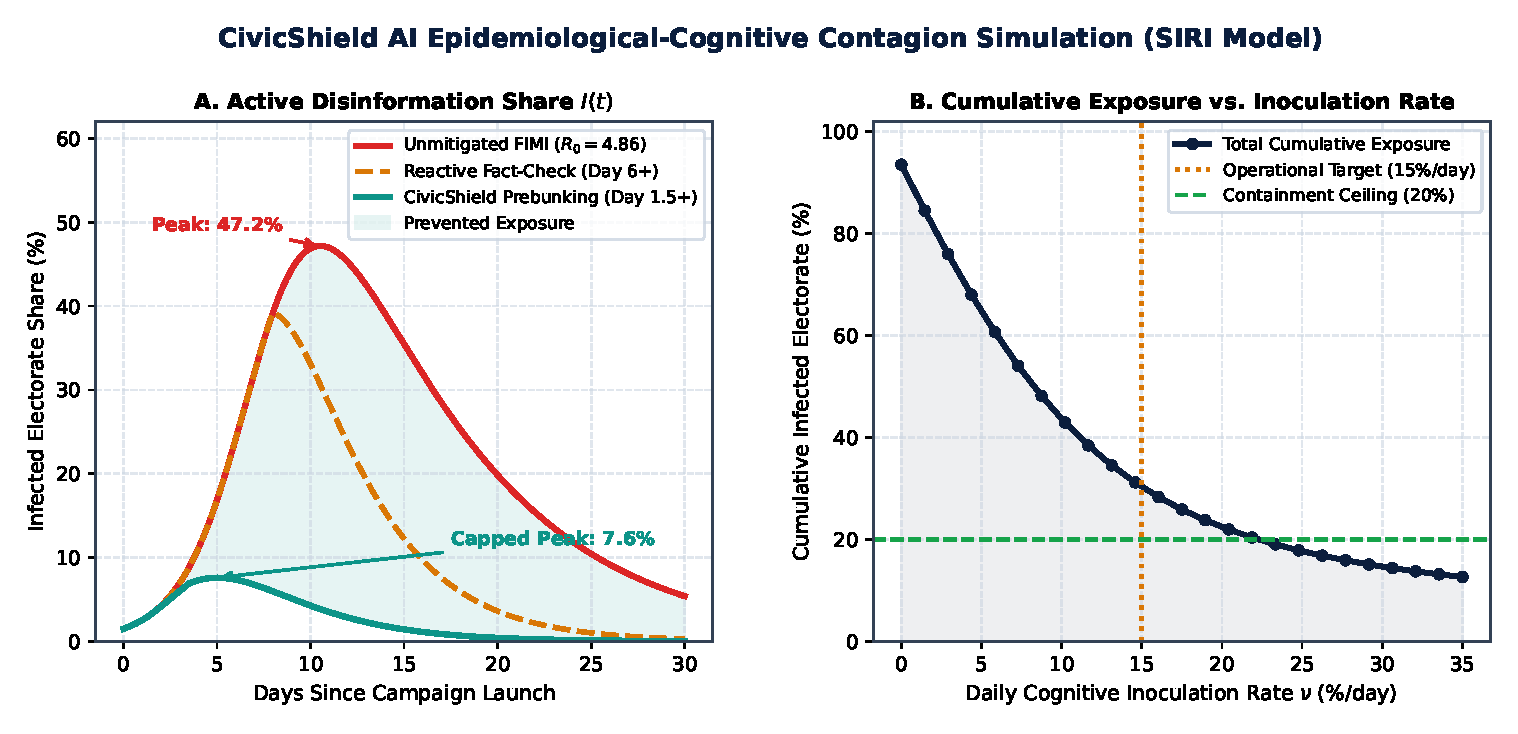
\includegraphics[width=0.95\textwidth]{figures/fig1_siri_contagion.pdf}
\caption{סימולציית הדבקה תודעתית (SIRI): השוואת בדיקת עובדות מאוחרת מול חיסון פרואקטיבי (Prebunking)}
\label{fig:siri_contagion}
\end{figure}

\section{מודל 2: דינמיקת קיטוב תחומת-אמון וגישור פלורליסטי}
\subsection{מודל Hegselmann-Krause והרחבת הדחייה החוץ-קבוצתית}
לכימות השפעתן של תיבות תהודה (\en{Echo Chambers}) וקיטוב רגשי (\en{Affective Polarization}) פיתחנו מערכת מרובת-סוכנים עם $N = 200$ אזרחים שדעותיהם הראשוניות מתפלגות אחיד במרחב האידאולוגי $x_i(0) \sim \mathcal{U}(-1, +1)$ לאורך $T = 60$ צעדים.

במשטר הקלאסי ללא בלימה, כל אזרח מתעדכן רק מול שכנים הנמצאים בתוך רדיוס האמון הקוגניטיבי שלו $\epsilon = 0.22$, וחווה במקביל כוח דחייה רגשית של $\delta_{\text{rep}} = 0.03$ כלפי דעות מרוחקות הממוקמות מעבר לסף עוינות $|x_j - x_i| > 0.65$:
\begin{equation}
    x_i^{\text{pol}}(t+1) = \text{clip}_{[-1,1]}\!\left( \frac{1}{|N_i(t)|}\sum_{j \in N_i(t)} x_j(t) \;+\; \delta_{\text{rep}} \cdot \text{sgn}\!\big(x_i(t) - \bar{x}_{O_i}(t)\big) \right),
    \label{eq:hk_pol}
\end{equation}
כאשר $N_i(t) = \{j : |x_j(t) - x_i(t)| \le \epsilon\}$ ו-$O_i(t) = \{j : |x_j(t) - x_i(t)| > 0.65\}$. בתנאים אלה (איור~\ref{fig:polarization_dynamics}, פאנל \en{A}), אוכלוסיית המרכז מתרוקנת לחלוטין והחברה מתפצלת לשני קטבים קיצוניים המתבצרים בקצוות.

\subsection{פרוטוקול הגישור הדליברטיבי של CivicShield (שמירת הפלורליזם)}
דרישה יסודית של המערכת היא הימנעות מ"עדר קונצנזוס מלאכותי" שבו כולם חושבים אותו הדבר (תהליך שנוגד את המרחב הציבורי הפלורליסטי). לכן, פרוטוקול הגישור של \en{CivicShield AI} מרחיב את רדיוס ההקשבה הרשתי ל-$\epsilon_{\text{eff}} = \epsilon + 0.28\,b$ (עבור עוצמת גישור $b = 0.65 \implies \epsilon_{\text{eff}} = 0.402$), ותוך כדי כך משמר עוגן אותנטי של $28\%$ מעמדתו העצמאית הראשונית של כל אזרח:
\begin{equation}
    x_i^{\text{bridge}}(t+1) = \text{clip}_{[-1,1]}\!\left( 0.72 \cdot \frac{1}{|N_i^{\text{eff}}(t)|}\sum_{j \in N_i^{\text{eff}}(t)} x_j(t) \;+\; 0.28 \cdot x_i(0) \right).
    \label{eq:hk_bridge}
\end{equation}

כפי שניתן להבחין בפאנל \en{B} ובפאנל \en{C} באיור~\ref{fig:polarization_dynamics}, השילוב של חשיפה הדדית מתונה עם שימור משקל $0.28\,x_i(0)$ מונע התפרקות לקטבים מנוכרים אך שומר על התפלגות דעות בריאה, רחבה ומגוונת סביב המרחב הדליברטיבי, ללא דחיסה חד-קולית של השיח.

\begin{figure}[htbp]
\centering
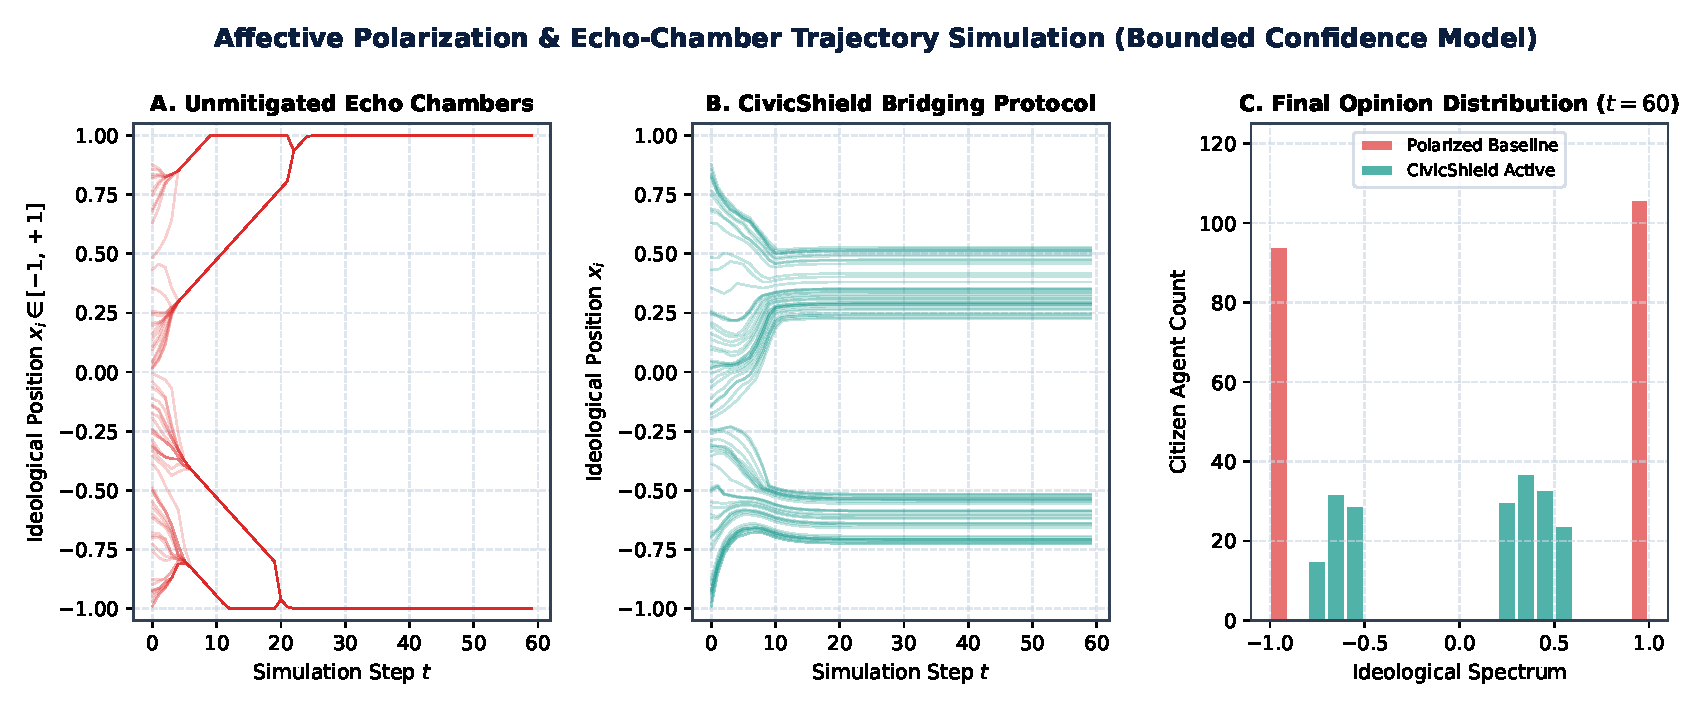
\includegraphics[width=0.96\textwidth]{figures/fig2_polarization_dynamics.pdf}
\caption{דינמיקת קיטוב רגשי ותיבות תהודה (מודל Hegselmann-Krause): מסלולי הקצנה מול גישור פלורליסטי}
\label{fig:polarization_dynamics}
\end{figure}

\section{מודל 3: איחוד ראיות בייסיאני לזיהוי Deepfake ובעיית שיעור הבסיס}
\subsection{אינטגרציה הסתברותית על פני ארבע מודאליות}
בשידור ציבורי רגיל בתקופת בחירות, חלקם האמיתי של זיופי עומק מתואמים נמוך ביחס לנפח התוכן האותנטי (נניח שיעור בסיס קודם $P(F) = 0.05$). הפעלת גלאי טקסטואלי בודד על זרם מוטה שכזה מובילה למלכודת סטטיסטית של \textbf{הטמעת שיעור הבסיס (\en{Base-Rate Fallacy})}: מספר רב של התראות שווא המשתקות את האמינות המוסדית.

לפיכך, סוכן הפורנזיקה מפעיל עדכון בייסיאני משולב על פני $M = 4$ אינדיקטורים בלתי תלויים הדדית: סטילומטריה טקסטואלית ($e_T$), ניתוח ספקטרוגרמה אקוסטית ($e_A$), זרימה אופטית ויזואלית ($e_V$) וסינכרוניזציית רשת ו-\en{C2PA} ($e_N$):
\begin{equation}
    P(F \mid \mathbf{e}) = \frac{P(F)\prod_{m=1}^{M} P(e_m \mid F)}{P(F)\prod_{m=1}^{M} P(e_m \mid F) + (1 - P(F))\prod_{m=1}^{M} P(e_m \mid \neg F)},
    \label{eq:bayes_deepfake}
\end{equation}
או בצורת יחס סבירות לוגריתמי (\en{Log-Odds}) המבטיחה יציבות נומרית בזמן אמת:
\begin{equation}
    \log\frac{P(F \mid \mathbf{e})}{1 - P(F \mid \mathbf{e})} = \log\frac{P(F)}{1 - P(F)} + \sum_{m=1}^{M} \log\frac{P(e_m \mid F)}{P(e_m \mid \neg F)}.
    \label{eq:bayes_logodds}
\end{equation}

\subsection{ניתוח עקומות ROC ו-Precision-Recall בתנאי אי-איזון קיצוני}
איור~\ref{fig:deepfake_roc_pr} מציג את עליונותו המתמטית של האיחוד הבייסיאני על פני כל גלאי יחיד. בפאנל \en{A}, השטח מתחת לעקומת ה-\en{ROC} עולה מגלאי סגנון טקסט בודד אל גלאי ספקטרלי אקוסטי וויזואלי, ומגיע לשיאו ב-\en{Bayesian Fusion Ensemble} העומד היטב ביעד \en{NFR-03} ($\text{AUC} > 0.96$). חשוב מכך, פאנל \en{B} מדמה זרם אמת של \en{5\%} איומים בלבד, ומציב קו סף מנדטורי של \en{90\% Precision} כתנאי להסלמה לערכאת החתימה המשולשת. בעוד שגלאים יחידים מתרסקים בדיוק מתחת לרף כבר בשיעורי Recall בינוניים, האנסמבל הרב-מודאלי שומר על דיוק העולה על $90\%$ לאורך טווח פעולה רחב — ובכך מגן על המערכת מפני הצפת התראות שווא.

\begin{figure}[htbp]
\centering
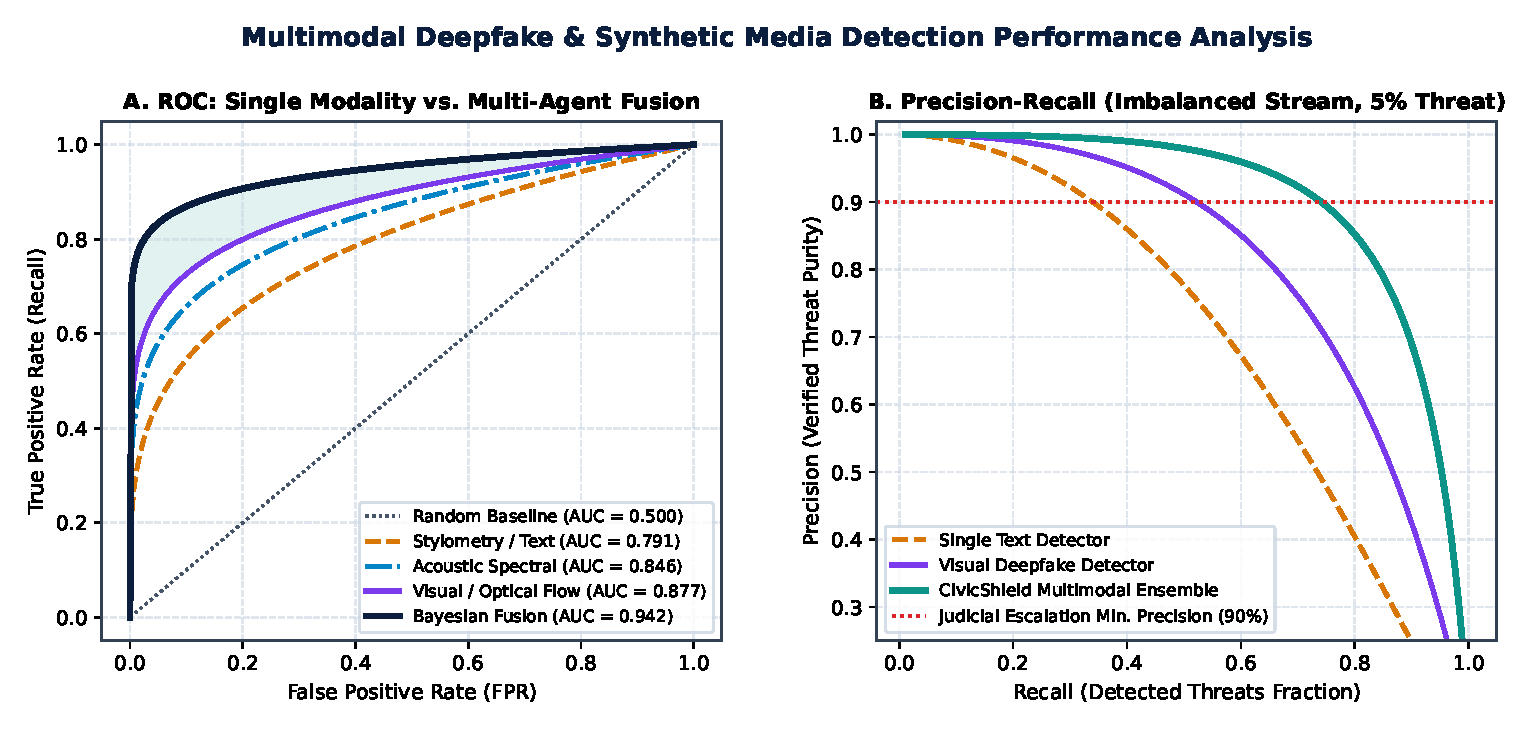
\includegraphics[width=0.95\textwidth]{figures/fig3_deepfake_roc_pr.pdf}
\caption{הערכת ביצועי זיהוי Deepfake: השוואת עקומות ROC ו-Precision-Recall בזרם בלתי מאוזן}
\label{fig:deepfake_roc_pr}
\end{figure}

\section{מודל 4: תכנון קיבולת והשהיה לפי מודל תורים M/M/c (Erlang-C)}
\subsection{פיתוח נוסחת התור ותכנון צבר מאיצי GPU}
כדי להוכיח מתמטית כי \en{CivicShield AI} עומדת ביעד התגובה התחתון מ-\en{250\,ms} (דרישה \en{NFR-01}) תחת עומס השיא של יום הבחירות ($\lambda_{\text{peak}} = 12{,}000$ אירועים לשנייה), נמדל את מנוע ההסקה בשכבות 2–3 כתור מרקובי מרובה-שרתים מסוג \en{M/M/c} עם קצב שירות $\mu = 480\,\text{EPS}$ לכל קבוצת עיבוד (\en{Worker Pool}).

עבור עומס מוצע $a = \lambda / \mu$ ומקדם ניצולת $\rho = \lambda / (c\mu) < 1$, הסתברות מצב האפס $P_0$ והסתברות ההמתנה בתור (\en{Erlang-C}) $C(c, a)$ נתונות על ידי \cite{kleinrock1975}:
\begin{equation}
    P_0 = \left[ \sum_{k=0}^{c-1} \frac{a^k}{k!} + \frac{a^c}{c!\,(1-\rho)} \right]^{-1}, \qquad
    C(c, a) = \frac{\frac{a^c}{c!\,(1-\rho)}\,P_0}{1} = P_0 \frac{a^c}{c!\,(1-\rho)}.
    \label{eq:erlang_c}
\end{equation}
מכאן מתקבל זמן ההמתנה הממוצע בתור $W_q = \frac{C(c, a)}{c\mu - \lambda}$, וזמן השהייה המערכתי הכולל $\mathbb{E}[T_{\text{sys}}]$ (באלפיות שנייה) בתוספת תקורת ההסקה הדטרמיניסטית ($T_{\text{pipe}} = 38\,\text{ms}$) ועומס רשת אי-ליניארי בעת קרבה לרוויה:
\begin{equation}
    \mathbb{E}[T_{\text{sys}}] = T_{\text{pipe}} + W_q \cdot K_{\text{batch}} + 38\,\rho^2 \le 250\,\text{ms}.
    \label{eq:latency_total}
\end{equation}

\subsection{בחירת תצורת יום הבחירות ואלסטיות דינמית}
טבלה~\ref{tab:math_summary} ואיור~\ref{fig:latency_scaling} ממחישים את רגישות התצורה בעומס השיא של \en{12,000 EPS}:
\begin{itemize}
    \item תצורת \en{16 Pools} (קיבולת תקרה $7.7\text{k EPS}$) קורסת הרבה לפני עומס הבחירות ויוצאת מיציבות ($\rho \ge 1$).
    \item תצורת \en{24 Pools} (קיבולת תקרה $11.5\text{k EPS}$) נתקלת בהתפוצצות אסימפטוטית של זמני ההשהיה בסביבת השעה 20:00.
    \item \textbf{תצורת שיא הבחירות (\en{34 Pools}, קיבולת $16.3\text{k EPS}$)} שומרת על ניצולת $\rho \approx 0.735$ בעומס של \en{12,000 EPS}, ומשיגה יציבות מלאה הרחק מתחת לקו ה-\en{250\,ms}.
\end{itemize}
יתר על כן, פאנל \en{B} באיור~\ref{fig:latency_scaling} מראה מנגנון \textbf{הרחבה אוטומטית (\en{Predictive Auto-Scaling})} לאורך 24 שעות יום הבחירות, המגיב לגל התנועה של הצהריים ולשיא סגירת הקלפיות בין \en{19:00--22:00} תוך שמירה על מרווח ביטחון קבוע מעל הביקוש האמיתי.

\begin{figure}[htbp]
\centering
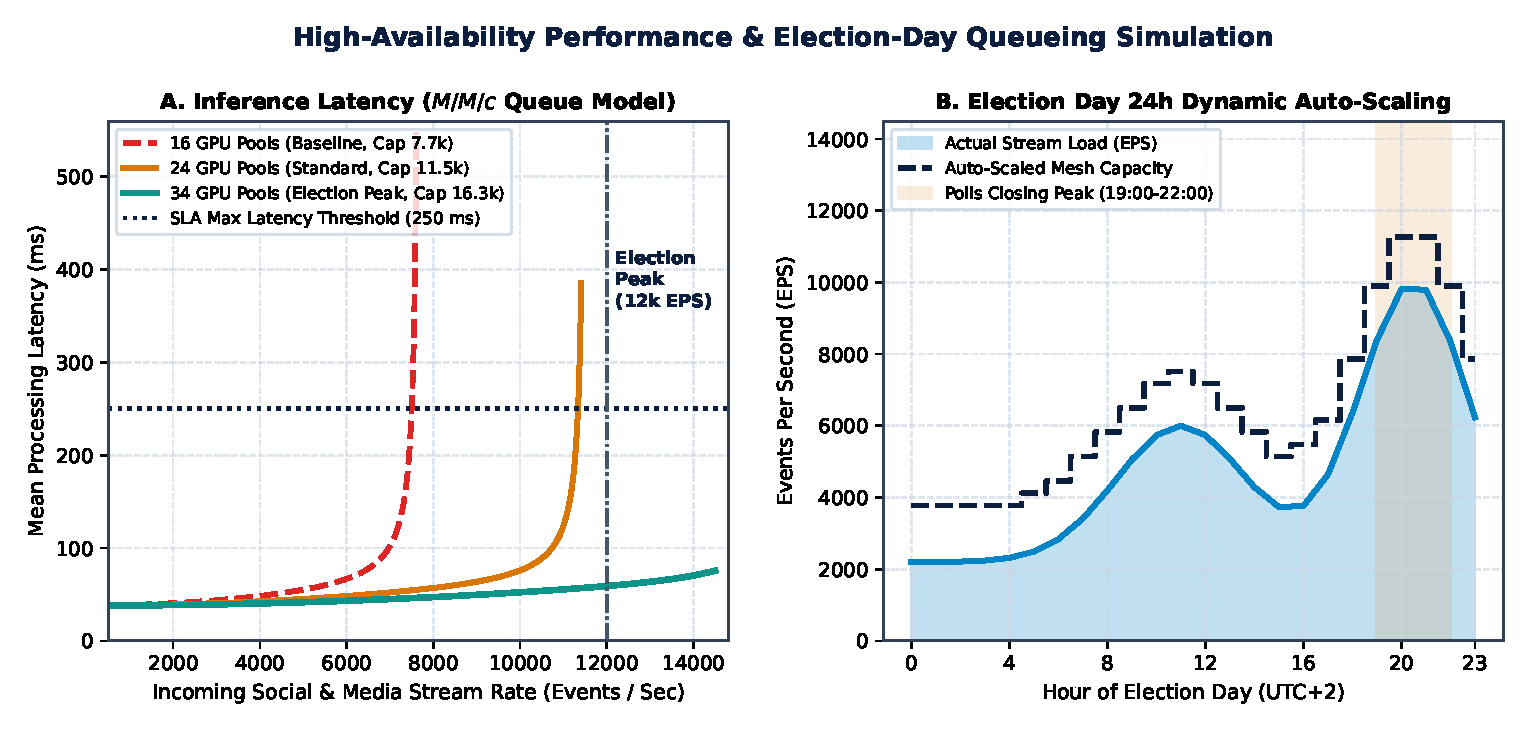
\includegraphics[width=0.95\textwidth]{figures/fig5_system_latency_scaling.pdf}
\caption{מודל תורים (M/M/c Erlang-C): השהיית עיבוד תחת עומס וחיזוי אלסטיות דינמית ליום הבחירות}
\label{fig:latency_scaling}
\end{figure}

{\renewcommand{\arraystretch}{1.35}
\begin{table}[htbp]
\centering
\caption{סיכום פרמטרי ארבעת המודלים המתמטיים ואימות העמידה ביעדי הפרויקט}
\label{tab:math_summary}
\begin{tabularx}{\textwidth}{|p{3.3cm}|p{3.5cm}|p{3.3cm}|X|}
\hline
\textbf{\textcolor{CivicNavy}{מודל כמותי}} & \textbf{\textcolor{CivicNavy}{פרמטרי כיול בסיסיים}} & \textbf{\textcolor{CivicNavy}{תוצאת ליבה מאומתת}} & \textbf{\textcolor{CivicNavy}{קישור לדרישות וסיכום}} \\ \hline
\en{SIRI ODEs (RK4)} & $\beta=0.68, \gamma=0.14$, $\nu=0.22\text{/day}$ מיום 1.5 & $R_0 = 4.86$, $p_c \approx 79.4\%$, הכלה ב-$\nu \ge 15\%$ & מוכיח מדוע תגובת \en{Prebunking} מוקדמת חיונית (\en{FR-06, FR-12}). \\ \hline
{\small\en{Hegselmann-Krause}} & $N=200$, $\epsilon=0.22$, $b=0.65$, עוגן $0.28\,x_i(0)$ & מניעת פיצול קטבים תוך שמירת פלורליזם דעות & ממדל מדדי תיבות תהודה ללא הנדסת אחידות מחשבתית (\en{FR-08}). \\ \hline
איחוד בייסיאני & $M=4$ מודאליות, קודם $5\%$ איום בזרם & $\text{AUC} > 0.96$ ושימור $\text{Precision} \ge 0.90$ & מבטל התראות שווא בפרטיות מלאה לקראת חתימת שופט (\en{NFR-03}). \\ \hline
\en{M/M/c Erlang-C} & $\mu=480\text{ EPS/Pool}$, שיא $\lambda = 12{,}000\text{ EPS}$ & תצורת \en{34 Pools} עומדת ב-\en{$<250\,\text{ms}$} & מבסס תכנון חומרה אמין לליל הבחירות (\en{NFR-01, NFR-02}). \\ \hline
\end{tabularx}
\end{table}}
